\documentclass{article}
\usepackage[utf8]{inputenc}
\usepackage{amsmath,amsthm,amssymb}
\usepackage{amsfonts}
\usepackage{arydshln}
\usepackage{enumitem}
\usepackage{float}
\usepackage{graphicx}
\usepackage{hyperref}
\usepackage{listings}
\usepackage{makecell}
\usepackage[margin=0.5in]{geometry}
\usepackage{multicol}
\usepackage{subcaption}
\usepackage{wrapfig}
\allowdisplaybreaks
\newtheorem{theorem}{Theorem}
\newtheorem{lemma}{Lemma}

\title{{\large Math 465}\\ Homework 01}
\author{Bridgette Delight}
\date{\today}

\begin{document}

\maketitle

\section{}
By following the steps of the proof of Theorem 1.1 and the proof of The Contraction Mapping Theorem, prove the following facts:

\begin{enumerate}[label = (\alph*)]
    \item the function $f(x)= \frac{1}{\sqrt{2}+0.5x}-1.5x$ has exactly one root in the interval $\left[0, \frac{1}{2}  \right]$,
    \item the sequence of approximations $\left\{ s_k \right\}^{\infty}_{k=0}$ defined recursively by 
    \begin{equation}\label{cases}
    \begin{cases}
    s_0 \in \left[0, \frac{1}{2} \right] - \text{arbitrary}\\
    s_{k+1} = \frac{2}{3\sqrt{2}+1.5s_k}, &k=0,1,2,\dots
    \end{cases}
    \end{equation}converges to the root.
\end{enumerate}


\vspace{10mm}

\subsection*{(a)}



\begin{align*}
    \text{To show that $f(x)$ has exactly 1 root, we first have to}&\\
    \text{show that a root exists to begin with. So, if}&\\
    f&:[a,b] \to \mathbb{R} \text{ is continuous and}\\
    [a,b] &= \left[0,\frac{1}{2}\right]\\
    \text{and,}&\\
    0 &\ge f(a) \cdot f(b)\\
    \text{then, }&\\
    &\exists \text{ } \xi \in [a,b] \text{ where, }f(\xi)=0 \\
    f(x)&= \frac{1}{\sqrt{2}+0.5x}-1.5x \text{ for }x \in \left[0,\frac{1}{2}\right] \\
    \text{We will use the intermediate value theorem to prove }&\\
    \text{that there is a 0 between $f(a)$ and $f(b)$ }&\\
    0 &\le f(a) \cdot f(b)\\
    f(a)&=f(1)>0\\
    f(b)&=f\left(\frac{1}{2}\right)<0 \\
    f(x) &= \frac{1}{\sqrt{2}+0.5x}-1.5x\\
    f(0)&= \frac{1}{\sqrt{2}+0}-0\\
    0&< \frac{1}{\sqrt{2}}=f(a)\\
    f\left(\frac{1}{2}\right) &= \frac{1}{\sqrt{2}+\frac{1}{2} \cdot \frac{1}{2}}-\frac{3}{2} \cdot \frac{1}{2}\\
    &= \frac{1}{0.25 + 1.414}-\frac{3}{4}\\
    0&> 0.60088 - .75 =f(b)\\
    \text{Therefore, a root exists in the interval $[a,b]$.}&\\
    \text{In order to show uniqueness we will say that since}&\\
    \text{$f(x)$ has a root, then there exists a}&\\
    g&:g(x)=0\\
    \Rightarrow f(x)&= g(x)-x=0\\
    \text{So,}&\\
    g(x)&= \frac{2}{3\sqrt{2}+1.5x}\\
    |x-y|&= |g(x)-g(y)|\\
    \text{From the Mean Value Theorem we get,}&\\
    |x-y|&\le |g(x)-g(y)|=|g'(z)(x-y)| \text{, while }z \in [x,y]\\
    g'(x) &= \frac{-3}{(3\sqrt{2}+1.5x)^2}\\
    \text{As $g(x)$ is a monotone decreasing function within the}&\\
    \text{bounds of $\left[0, \frac{1}{2}\right]$ we can find the upper bound.}&\\
    g'(0)&= \frac{1}{6}\\
    \Rightarrow |x-y|&= |g(x)-g(y)| \le \frac{x-y}{6}\\
    \text{Therefore $g$ is a contraction.}&\\
    \text{To show that the root is unique we will use a proof}&\\
    \text{by contradiction.}&\\
    \text{We make the assumption that there exists}&\\
    \text{two fixed points $\eta$ and $\xi$. So,}&\\
    |\xi - \eta|&= |g(\xi)-g(\eta)|\le \bigg | \frac{\xi - \eta}{6}\bigg |\\
    \Rightarrow |\xi - \eta|& \le \bigg | \frac{\xi - \eta}{6}\bigg |\\
    \Rightarrow \frac{| \xi - \eta|}{\xi - \eta|}& \le \frac{1}{6}\\
    \text{Which means, }&, \le \frac{1}{6}\\
    \text{Which is wrong. Thus, it is a contradiction meaning}&\\
    \text{that there exists only one fixed point for $g$.}
\end{align*}

\vspace{10mm}
\subsection*{(b)}

\begin{align*}
     s_{k+1} &= \frac{2}{3\sqrt{2}+1.5s_k} \text{, }k=0,1,2,\dots\\
     s_0 &\in \left[0, \frac{1}{2} \right]\\
\end{align*}



\section{}
Take $s_0 = \frac{1}{\sqrt{6}}$ in (\ref{cases}) and write a code that you can use to compute the first 10000 elements of the sequence $\left\{ s_k \right\}^{\infty}_{k=0}$.
\vspace{10mm}


Here is the code in python. It will return a data frame from $s_0\to s_10000$ :
\begin{verbatim}
    def Sk(n):
    sequence = [0, (1/math.sqrt(6))]
    q = 3*math.sqrt(2)
    for index in range(n):
        sequence.append(2/(q+1.5*sequence[-1]))
    return sequence

    df = pd.DataFrame(Sk(10000))
    df = df.iloc[1:]
    df = df.reset_index(drop=True)
    df
\end{verbatim}

\begin{table}[H]
    \centering
    \begin{tabular}{|r|c|}
        \Xhline{1 pt}
         \textbf{k}& \textbf{$s_k$}  \\
         \Xhline{1.5 pt}
         0 & 0.4082482904638631\\
         \Xhline{1 pt}
         1 & 0.4119453334948641\\
         \Xhline{1 pt}
         2 & 0.41147533208484804\\
         \Xhline{1 pt}
         3 & 0.4115350233838435\\
         \Xhline{1 pt}
         $\vdots$ & $\vdots$\\
          \Xhline{1 pt}
         9,999 & 0.4115282959774586\\
          \Xhline{1 pt}
         10,000 & 0.4115282959774586\\
         \Xhline{1 pt}
    \end{tabular}
    \caption{Abbreviated table for the sequence $\left\{ s_k\right\}_{k=0}^{10000}$}
    \label{tab:10sequence}
\end{table}


\section{}
Determine a formula for the exact value of the root $\xi \in \left[0,\frac{1}{2} \right]$ of the function $f$.
\vspace{10mm}


\section{}
Run your code and present a table that displays the iteration number $k \in {1,2,\dots,15}$ in the first column, the corresponding approximations $s_k$ in the second column, and the corresponding errors of the approximations in the third column.
\vspace{10mm}

\begin{table}[H]
    \centering
    \begin{tabular}{|r|l|c|}
        \Xhline{1 pt}
         \centering \textbf{k}& \textbf{$s_k$}& \textbf{Error}  \\
         \Xhline{1.5 pt}
         0 & 0.4082482904638631&$3.280006\cdot e^{-03}$\\
         \Xhline{1 pt}
         1 & 0.4119453334948641&$4.170375\cdot e^{-04}$\\
         \Xhline{1 pt}
         2 & 0.41147533208484804&$5.296389\cdot e^{-05}$\\
         \Xhline{1 pt}
         3 & 0.4115350233838435&$6.727406\cdot e^{-06}$\\
         \Xhline{1 pt}
         4 & 0.41152744148658515 &$8.544909\cdot e^{-07}$\\
         \Xhline{1 pt}
         5 & 0.41152840451205874 & $1.085346\cdot e^{-07}$\\
          \Xhline{1 pt}
         6 & 0.41152828219175736 & $1.378570\cdot e^{-08}$\\
          \Xhline{1 pt}
         7 & 0.41152829772847227 &$2.224078\cdot e^{-09}$\\
          \Xhline{1 pt}
         8 & 0.41152829575505073 &$2.824962\cdot e^{-10}$\\
          \Xhline{1 pt}
         9 & 0.4115282960057081 &$3.588019\cdot e^{-11}$\\
          \Xhline{1 pt}
         10 & 0.4115282959738705 &$3.588019\cdot e^{-12}$\\
          \Xhline{1 pt}
         11 & 0.41152829597791435 &$4.558576\cdot e^{-13}$\\
          \Xhline{1 pt}
         12 & 0.41152829597740076 &$5.773160\cdot e^{-14}$\\
          \Xhline{1 pt}
         13 & 0.411528295977466 &$7.494005\cdot e^{-15}$\\
          \Xhline{1 pt}
         14 & 0.4115282959774577&$7.771561\cdot e^{-16}$\\
          \Xhline{1 pt}
         15 & 0.41152829597745877&$2.775558\cdot e^{-16}$\\
         \Xhline{1 pt}
    \end{tabular}
    \caption{Values for the sequence$\left\{ s_k\right\}_{k=0}^{15}$}
    \label{tab:15sequence}
\end{table}

\section{}
Present a figure showing the approximations $s_k$ (vertical axis) versus the iteration index $k$ (horizontal axis) for $k=1,2,\dots,15$.
\vspace{10mm}

\begin{figure}[H]
    \centering
    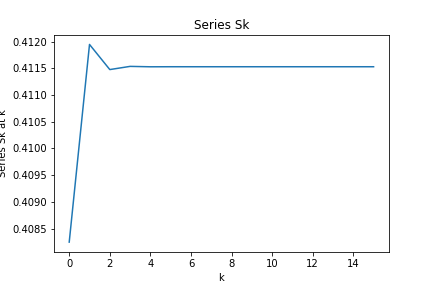
\includegraphics[width = .7\linewidth]{images/hw01q05.png}
    \caption{Figure}
    \label{fig:my_label}
\end{figure}


\section{}
Present a figure showing the errors $|s_k - \xi|$ of the approximations (vertical axis) versus the iteration index $k$ (horizontal axis) for $k=1,2,\dots,15$.
\vspace{10mm}



\section{}
For any $s_0 \in \left[0, \frac{1}{2} \right]$, derive an upper bound on the number of iteration $k$ required to ensure that the $k^{th}$ iterate $s_k$ is correct to six decimal digits. Shows all steps of your derivation. Write down the value of the upper bound in case $s_0 = \frac{1}{\sqrt{6}}$.
\vspace{10mm}

\section{}
Run your code with $s_0 \in \left[0,\frac{1}{\sqrt{6}} \right]$ and find the index $i$ of the first iterate $s_i$ that is correct to six decimal digits. Compare this to your answer to question 7. Is this what you have expected? Why?
\vspace{10mm}





\end{document}